\documentclass[tikz,border=12pt]{standalone}
\usepackage{tikz}
\usetikzlibrary{positioning, arrows.meta, calc}

% Corpus slab colors
\definecolor{prose}{RGB}{70, 130, 180}
\definecolor{html}{RGB}{60, 179, 113}
\definecolor{code}{RGB}{218, 165, 32}
\definecolor{md}{RGB}{200, 110, 110}
\definecolor{json}{RGB}{178, 102, 178}

% Stage frame colors
\definecolor{corpus}{RGB}{90, 130, 175}
\definecolor{base}{RGB}{95, 110, 165}
\definecolor{loss}{RGB}{200, 90, 70}
\definecolor{final}{RGB}{60, 165, 110}

\begin{document}
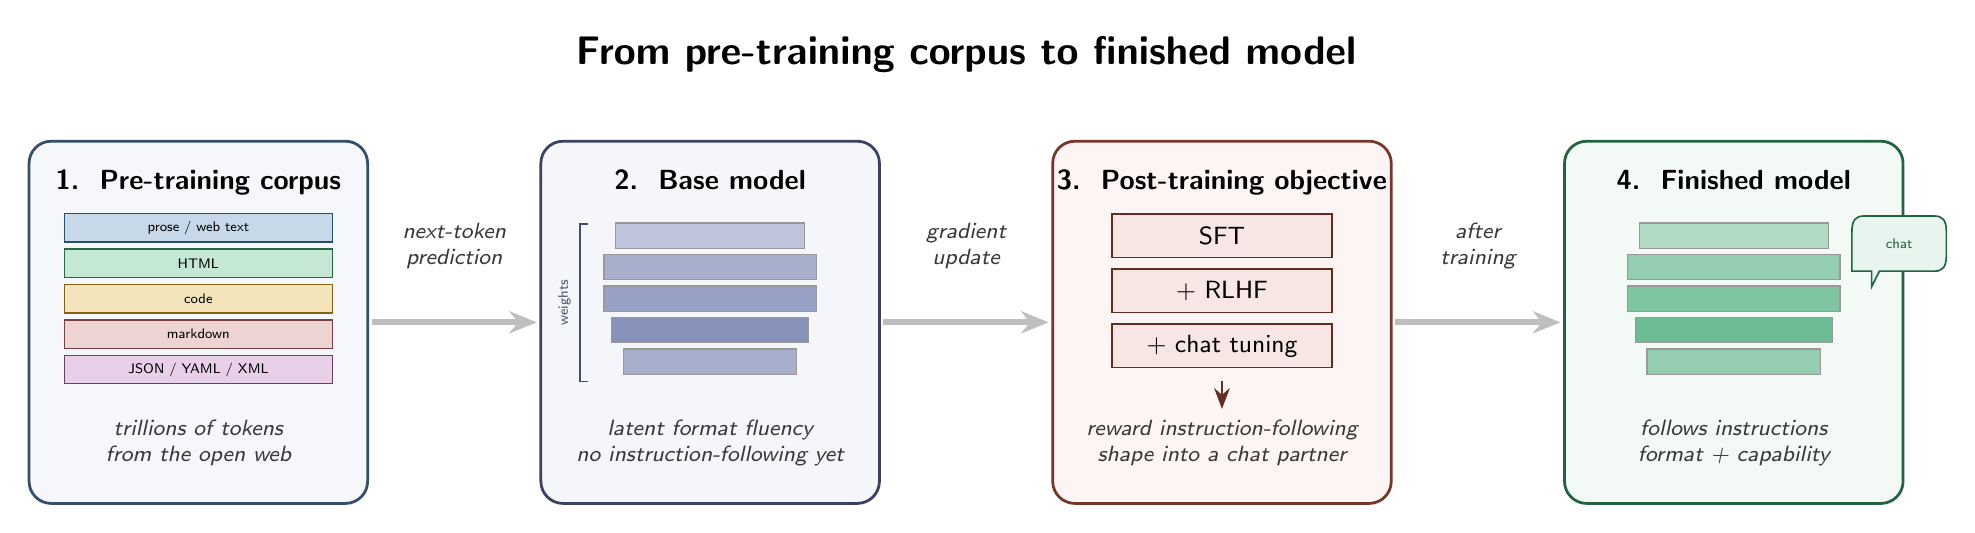
\begin{tikzpicture}[
    >=Stealth,
    font=\sffamily,
    stagebox/.style={
        rectangle, rounded corners=8pt,
        draw=#1!60!black, fill=#1!6,
        line width=1pt,
        minimum width=4.3cm, minimum height=4.6cm,
    },
    stagetitle/.style={font=\sffamily\bfseries},
    caption/.style={
        font=\sffamily\footnotesize\itshape, text=gray!45!black,
        align=center,
    },
    flow/.style={
        -{Stealth[length=10pt, width=8pt]},
        line width=2.2pt, draw=gray!50,
    },
    layer/.style={
        rectangle, fill=#1, draw=black!40,
        line width=0.5pt, minimum height=0.32cm,
    },
    slab/.style={
        rectangle, fill=#1!30, draw=#1!60!black,
        line width=0.5pt, font=\sffamily\tiny,
        minimum height=0.36cm, minimum width=3.4cm,
        inner sep=2pt, align=center,
    },
    obj/.style={
        rectangle, fill=loss!15, draw=loss!50!black,
        line width=0.6pt, minimum width=2.8cm, minimum height=0.55cm,
        font=\sffamily\small, align=center,
    },
]

% =============== Title ===============
\node[font=\sffamily\Large\bfseries] at (0, 3.4)
    {From pre-training corpus to finished model};

% Stage center x-coordinates (gap of 6.5cm - 4.3cm box width = 2.2cm
% of clearance between stages, enough for an arrow + multi-line label).
\def\sa{-9.75}
\def\sb{-3.25}
\def\sc{3.25}
\def\sd{9.75}

% =============== STAGE 1: Pre-training corpus ===============
\node[stagebox=corpus] at (\sa, 0) {};
\node[stagetitle, anchor=north] at (\sa, 2.05) {1.~~Pre-training corpus};
\node[slab=prose] at (\sa,  1.20) {prose / web text};
\node[slab=html]  at (\sa,  0.75) {HTML};
\node[slab=code]  at (\sa,  0.30) {code};
\node[slab=md]    at (\sa, -0.15) {markdown};
\node[slab=json]  at (\sa, -0.60) {JSON / YAML / XML};
\node[caption, anchor=south] at (\sa, -1.95)
    {trillions of tokens\\from the open web};

% =============== STAGE 2: Base model ===============
\node[stagebox=base] at (\sb, 0) {};
\node[stagetitle, anchor=north] at (\sb, 2.05) {2.~~Base model};
\node[layer=base!40, minimum width=2.4cm] at (\sb,  1.10) {};
\node[layer=base!55, minimum width=2.7cm] at (\sb,  0.70) {};
\node[layer=base!65, minimum width=2.7cm] at (\sb,  0.30) {};
\node[layer=base!75, minimum width=2.5cm] at (\sb, -0.10) {};
\node[layer=base!55, minimum width=2.2cm] at (\sb, -0.50) {};
% Bracket on the left labelling 'weights'
\draw[base!70!black, line width=0.6pt]
    (\sb-1.55, -0.75) -- (\sb-1.65, -0.75)
    -- (\sb-1.65,  1.25) -- (\sb-1.55,  1.25);
\node[font=\sffamily\tiny, text=base!70!black, rotate=90]
    at (\sb-1.85, 0.25) {weights};
\node[caption, anchor=south] at (\sb, -1.95)
    {latent format fluency\\no instruction-following yet};

% =============== STAGE 3: Post-training objective ===============
\node[stagebox=loss] at (\sc, 0) {};
\node[stagetitle, anchor=north] at (\sc, 2.05) {3.~~Post-training objective};
% Boxed list of training stages
\node[obj] at (\sc,  1.10) {SFT};
\node[obj] at (\sc,  0.40) {$+$ RLHF};
\node[obj] at (\sc, -0.30) {$+$ chat tuning};
% Down arrow indicating training pressure
\draw[->, loss!50!black, line width=1pt] (\sc, -0.75) -- (\sc, -1.10);
\node[caption, anchor=south] at (\sc, -1.95)
    {reward instruction-following\\shape into a chat partner};

% =============== STAGE 4: Finished model ===============
\node[stagebox=final] at (\sd, 0) {};
\node[stagetitle, anchor=north] at (\sd, 2.05) {4.~~Finished model};
\node[layer=final!40, minimum width=2.4cm] at (\sd,  1.10) {};
\node[layer=final!55, minimum width=2.7cm] at (\sd,  0.70) {};
\node[layer=final!65, minimum width=2.7cm] at (\sd,  0.30) {};
\node[layer=final!75, minimum width=2.5cm] at (\sd, -0.10) {};
\node[layer=final!55, minimum width=2.2cm] at (\sd, -0.50) {};
% Small chat indicator: a speech bubble built from primitives
\draw[final!60!black, fill=final!12, line width=0.6pt]
    (\sd+1.50, 0.65)
        -- (\sd+1.50, 1.15)
        .. controls (\sd+1.50, 1.30) and (\sd+1.55, 1.35) .. (\sd+1.65, 1.35)
        -- (\sd+2.55, 1.35)
        .. controls (\sd+2.65, 1.35) and (\sd+2.70, 1.30) .. (\sd+2.70, 1.15)
        -- (\sd+2.70, 0.85)
        .. controls (\sd+2.70, 0.70) and (\sd+2.65, 0.65) .. (\sd+2.55, 0.65)
        -- (\sd+1.85, 0.65)
        -- (\sd+1.75, 0.45)
        -- (\sd+1.75, 0.65)
        -- cycle;
\node[font=\sffamily\tiny, text=final!55!black]
    at (\sd+2.10, 1.00) {chat};
\node[caption, anchor=south] at (\sd, -1.95)
    {follows instructions\\format + capability};

% =============== Flow arrows between stages ===============
\draw[flow] ($(\sa, 0)+(2.20, 0)$) -- ($(\sb, 0)+(-2.20, 0)$);
\draw[flow] ($(\sb, 0)+(2.20, 0)$) -- ($(\sc, 0)+(-2.20, 0)$);
\draw[flow] ($(\sc, 0)+(2.20, 0)$) -- ($(\sd, 0)+(-2.20, 0)$);

% Arrow labels above each arrow
\node[caption, anchor=south]
    at ($(\sa, 0.55)!0.5!(\sb, 0.55)$) {next-token\\prediction};
\node[caption, anchor=south]
    at ($(\sb, 0.55)!0.5!(\sc, 0.55)$) {gradient\\update};
\node[caption, anchor=south]
    at ($(\sc, 0.55)!0.5!(\sd, 0.55)$) {after\\training};

\end{tikzpicture}
\end{document}
